\documentclass{beamer}
\useinnertheme{rectangles}
\usepackage{graphicx}
\usepackage{epsfig}
\usepackage{mydef}
%\usepackage{MinionPro}
\usepackage{mathptm}
\usefonttheme{serif}

\title{AllJoyn Overview}
\author{}
\date{\today}
\begin{document}

\begin{frame}
\titlepage
\end{frame}


\begin{frame}
\frametitle{Overview of AllJoyn}

\bb{What is AllJoyn?}
\bit
\w A software infrastructure for distributed applications.
\w It has the form of a library.
\w Provides API with which users can write a program.
\eit

\vspace*{0.3cm}

\bb{Which abstraction does AllJoyn adopt?}
\bit
\w It's mostly based on two abstractions:
  \bit
  \w PULL: Method invocation
  \w PUSH: Signal notification 
  \eit
\eit

\vspace*{0.3cm}

\bb{How is it AllJoyn Implemented}
\bit
\w Method invocation and signal notification are implemented 
   using \bb{message bus}.
\eit

\bb{Where is AllJoyn located}
\bit
\w Sits between OS and user application.
\eit
\end{frame}

\begin{frame}
\frametitle{Component of AllJoyn Framework}
\end{frame}

\begin{frame}
\frametitle{Architecture of AllJoyn Framework}

%\DeclareGraphicsExtensions{.jpg}
\bb{Static architecture}
\centerline{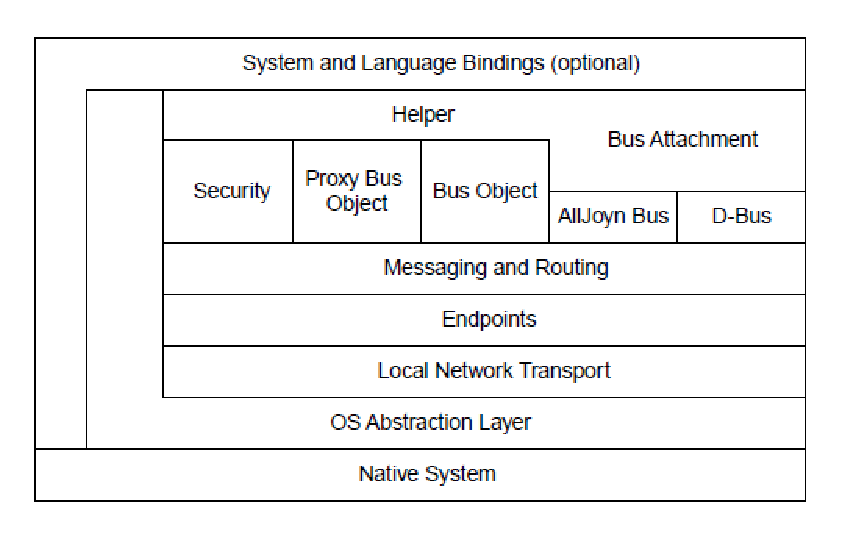
\includegraphics[height=3.5cm,width=6cm]{aj}}

\bb{Runtime architecture}
\centerline{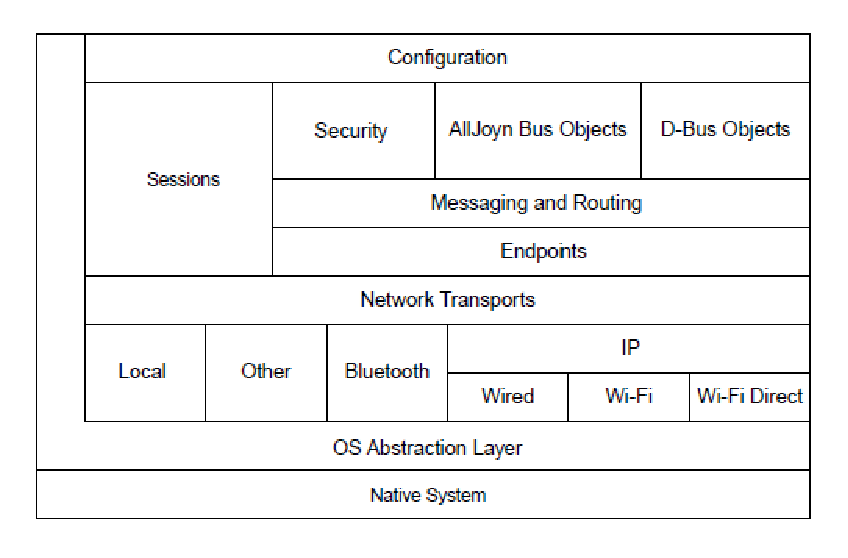
\includegraphics[height=3.5cm,width=6cm]{ajd}}


\end{frame}

\begin{frame}
\frametitle{Distributed services}
\bb{Three essential functionalities}
\bit
\w Discovery
\w Announcement
\w Service: Pull-based and Push-based
\eit
\end{frame}

\begin{frame}
\frametitle{Session vs Sessionless (i.e. Request/Reply)}
\end{frame}

\begin{frame}
\frametitle{Issue: Naming}
\end{frame}

\begin{frame}
\frametitle{Issue: Discovery}
\end{frame}

\begin{frame}
\frametitle{Issue: Announcement}
\end{frame}

\begin{frame}
\frametitle{Issue: Fault Tolerance}
\end{frame}

\begin{frame}
\frametitle{Issue: Consistency}
\end{frame}

\begin{frame}
\frametitle{Issue: Atomicity}
\end{frame}

\begin{frame}
\frametitle{Issue: Security}
\end{frame}

\begin{frame}
\frametitle{Issue: Performance}
\end{frame}

\begin{frame}
\frametitle{Limitation of AllJoyn}
\bit
\w \bb{Inheritance-based}: CORBA is inheritance-based while Spring was composition-based.
\w \bb{Not symmetric}: full-fledged pull-service; half-baked push-service
(notification/signal)
\w \bb{Tied to object model}: good but why; message is more generic and more
   efficient.  
\eit
\end{frame}



\end{document}

%%  LocalWords:  RFID DSMS SQL CEP IFP Dataflow cep compsys softsys
